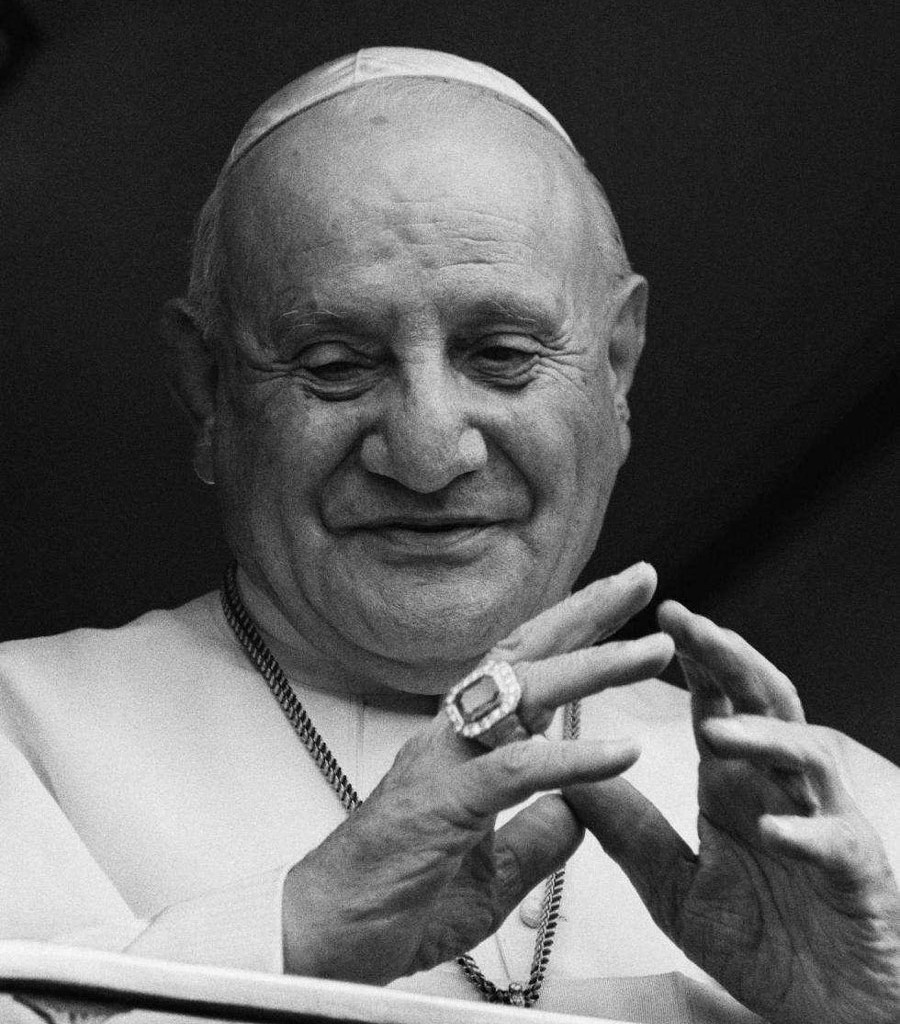
\includegraphics{papa.jpg}

Papa Giovanni XXIII, eletto nel 1958, si impegnò con determinazione in un vasto rinnovamento della Chiesa per rendere questa Istituzione più vicina alla gente e attenta alla giustizia e all’esigenza dei popoli.

Nei suoi cinque anni di Pontificato riuscì ad avviare il rinnovato impulso della Chiesa Universale.

E’ ricordato con l’appellativo di “Papa buono”.

Ebbe rapporti fraterni con i rappresentanti di diverse confessioni Cristiane e non Cristiane, rendendo  quindi più vicini tutti i popoli del mondo.

Nel 1962, dopo l’apertura del Concilio Ecumenico, il Presidente degli Stati Uniti d’America, J.F. Kennedy, annuncia alla Nazione la presenza di installazioni missilistiche a Cuba e l’avvicinamento all’isola di alcune navi sovietiche con a bordo le testate nucleari per l’armamento dei missili. Il mondo sembra precipitare nel baratro di un conflitto nucleare. Il Presidente Statunitense impone un blocco navale militare a 800 miglia dall’isola, ordinando agli equipaggi di essere pronti ad ogni eventualità, ma le navi sovietiche sembrano intenzionate a forzare il blocco.

Di fronte alla drammaticità della situazione, il Papa sente la necessità di agire per la pace. Il 25 ottobre successivo, alla Radio Vaticana, rivolge “a tutti gli uomini di buona volontà” un messaggio in lingua francese:

“Alla Chiesa sta a cuore più di ogni altra cosa la pace e la fraternità tra gli uomini; ed essa opera senza stancarsi mai a consolidare questi beni.  A questo proposito, abbiamo ricordato i gravi di coloro che portano la responsabilità del potere. Oggi noi rinnoviamo questo appello accorato e supplichiamo i Capi di Stato di non restare insensibili a questo grido dell’umanità. Facciano tutto ciò che è in loro potere per salvare la pace: così eviteranno al mondo gli orrori di una guerra di cui nessuno può prevedere le spaventevoli conseguenze.
Continuino a trattare…”.

Il messaggio suscita consenso in entrambe le parti in causa e, alla fine, la crisi rientra.
